\documentclass{article}
\usepackage[utf8]{inputenc}
\usepackage{amsmath}
\usepackage{float}
\usepackage{listings}
\usepackage[pdftex]{graphicx}
\usepackage{amssymb}
\usepackage{subcaption}
\usepackage{cancel}
\usepackage{float}

\DeclareMathOperator{\sech}{sech}
%---------------------------------------------------------
\author{Pratik Aghor}
\title{HW $\# 3$: Thin-film Flows and Inertia-less Convection}
\date{\today}  % Toggle commenting to test

\begin{document}

\maketitle
%----------------------------------------------
\section{Q $1$: Adhesive force in a ‘squeeze film’:}
%----------------------------------------------
\begin{figure}[H]
    \centering
    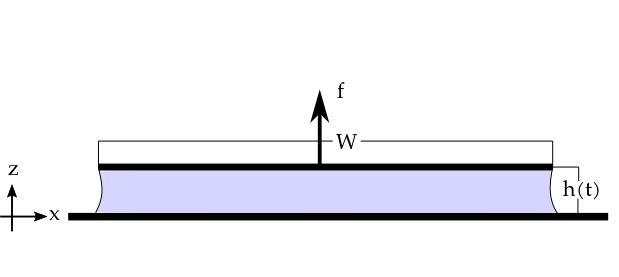
\includegraphics[scale = 0.5]{Figs/thin_film_knife.png}
    \caption{Thin film beneath a knife}
    \label{fig:thin_film_knife}
\end{figure}

Thin-film equations are valid here.
\begin{align}\label{eq:thin_film_dim}
 \begin{split}
  & \frac{\partial p}{\partial x} = \mu\frac{\partial^{2}u}{\partial z^{2}},\\
  %
  & \frac{\partial p}{\partial z} = \mu\frac{\partial^{2}w}{\partial z^{2}},\\
  %
  & \frac{\partial u}{\partial x} + \frac{\partial w}{\partial z} = 0.
 \end{split}
\end{align}
Let $x\sim W, z \sim h_{0}, u \sim U, p \sim P$. The continuity equation demands $\frac{\partial u}{\partial x}$ and $\frac{\partial w}{\partial z}$ to balance each other, hence $U/L \sim \tilde{W}/h$, giving a scale for $w$ in terms of $U$, i.e., $\tilde{W} \sim Uh_{0}/L = U\epsilon$.\\
The $x$-momentum equation gives $P$ in terms of $U$. 
$\frac{P}{W} \sim \frac{\mu U}{h_{0}^{2}}$, giving $P \sim \frac{\mu U W}{h_{0}^{2}} = \mu U/(\epsilon^{2}W)$.

The dimensionless equations then become:
\begin{align}\label{eq:thin_film_dimless}
 \begin{split}
  & \frac{\partial p}{\partial x} =\frac{\partial^{2}u}{\partial z^{2}},\\
  %
  & \frac{\partial p}{\partial z} = \epsilon^{2}\frac{\partial^{2}w}{\partial z^{2}},\\
  %
  & \frac{\partial u}{\partial x} + \frac{\partial w}{\partial z} = 0,
 \end{split}
\end{align}
where all the terms are now dimensionless.
The boundary conditions (BCs) are:
\begin{align}\label{eq:thin_film_bcs_dimless}
 \begin{split}
  &u = w = 0 \quad \textrm{at } z = 0, \\
  %
  &u = 0 \quad \textrm{at }z = h, \\
  & w = \partial_{t} h + u \partial_{x}h \quad \textrm{at }z = h\\
  & w = \partial_{t}h  \quad \textrm{using }u = 0 \quad \textrm{at } z = h,\\
  & p = p_{0} \quad \textrm{at }x = 0, 1.
 \end{split}
\end{align}

The leading order $z$-momentum equation ($\partial_{z}p = 0$) tells us that $p$ is not a function of $z$, i.e., $p \equiv p(x, t)$. Integrating the $x$-momentum equation wrt z, obtain 
\begin{align}\label{eq:thin_film_u}
 \begin{split}
  & \frac{\partial u}{\partial z} = \frac{\partial p}{\partial x} \int_{0}^{z} dz \\
  & \frac{\partial u}{\partial z} = \frac{\partial p}{\partial x} z + c_{1}(x, t)\\
  \Rightarrow \quad & u = \frac{\partial p}{\partial x} \frac{z^{2}}{2} + c_{1}(x, t) z + c_{2}(x, t)\\
  & u = 0 \quad \textrm{at z = }0, h, \\
  & c_{2} = 0 \\
  & c_{1} = - \frac{\partial p}{\partial x} \frac{h}{2}\\
  & \boxed{u = \frac{1}{2}\frac{\partial p}{\partial x}\left[z^{2}-hz \right]}.
 \end{split}
\end{align}

Integrating the continuity equation across the domain wrt $z$:
\begin{align}\label{eq:integrate_conti}
\begin{split}
 &\int_{z=0}^{h(x)} [\partial_{x} u + \partial_{z} w_{z} = 0 ] dz,\\
 %
 & w\big|_{0}^{h} + \int_{z=0}^{h(x)} \partial_{x} u dz = 0,\\
 %
 & \partial_{t}h + u|_{h} \partial_{x}h - 0 +  \int_{z=0}^{h(x)} (\partial_{x} u )dz = 0 \quad \hdots \textrm{using BCs for } w, \\
 %
 & \partial_{t}h + \cancel{u|_{h} \partial_{x}h} + \partial_{x} \int_{z=0}^{h(x)} u dz - \cancel{u|_{h} \partial_{x}h} = 0 \quad \hdots \textrm{Leibniz rule},\\
 %
 & \partial_{t}h + \partial_{x}\left[\int_{z=0}^{h(x)} u dz\right] = 0\\
 % 
 &\frac{dh}{dt} + \partial_{x}\left[\frac{1}{2}\frac{\partial p}{\partial x}\left[z^{3}/3-hz^{2}/2 \right]_{0}^{h} \right] = 0\\
 %
 &\frac{dh}{dt} - \partial_{x}\left[\frac{1}{2}\frac{\partial p}{\partial x}\frac{h^{3}}{6} \right] = 0\\
 %
 &\frac{dh}{dt} -\frac{h^{3}}{12}\frac{\partial^{2}p}{\partial x^{2}} = 0 \quad \hdots h \equiv h(t) \textrm{ only.} 
\end{split}
\end{align}

Integrating twice wrt $x$, we get $p$. 
\begin{align}\label{eq:thin_film_p}
 \begin{split}
  & p = \frac{12}{h^{3}}\frac{dh}{dt} \frac{x^{2}}{2} + c_{1}x + c_{2}\\
  & p = p_{0} \quad \textrm{at }x = 0, 1, \\
  %
  & c_{2} = p_{0}\\
  % 
  &c_{1} =-\frac{6}{h^{3}}\frac{dh}{dt} \\
  %
  & p - p_{0} = \frac{6}{h^{3}}\frac{dh}{dt}(x^{2}-x)
 \end{split}
\end{align}
%
\begin{figure}[H]
    \centering
    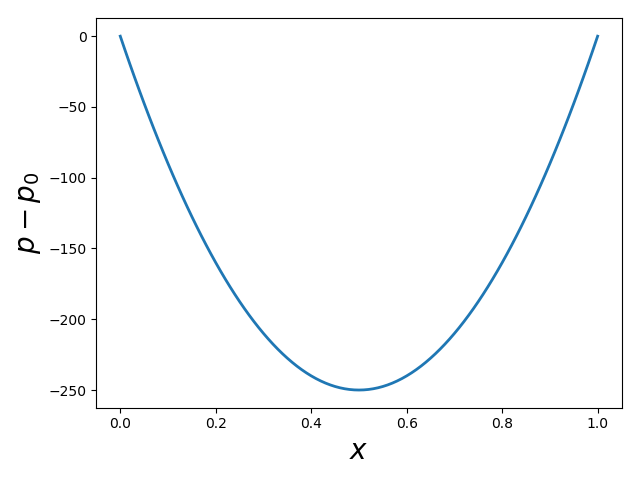
\includegraphics[scale = 0.5]{Figs/knife_gauge_p.png}
    \caption{Gauge pressure $p-p_{0}$ in the film}
    \label{fig:knife_gauge_p}
\end{figure}
%
Force per unit length (into the paper) exerted by the fluid on the knife is 

\begin{align}\label{eq:thin_film_force}
 \begin{split}
  & f_{1} = \int_{0}^{1} (p - p_{0}) dx, \\
  & f_{1} = \frac{6}{h^{3}}\frac{dh}{dt} \int_{0}^{1}(x^{2}-x) dx\\
  & f_{1} = \frac{6}{h^{3}}\frac{dh}{dt} \left[\frac{x^{3}}{3} - \frac{x^{2}}{2}\right]_{0}^{1}\\
  & f_{1} = -\frac{1}{h^{3}}\frac{dh}{dt}
 \end{split}
\end{align}

Therefore, the force (per unit length into the plane of paper) needed to pull the knife upward is $f = -f_{1} = \frac{1}{h^{3}}\frac{dh}{dt}$, which is huge if dimensionless $h \sim \epsilon$ is small.

%----------------------------------------------
\section{Q $2$:  Static shape of a pendant droplet with uniform surface tension and gravity:}
%----------------------------------------------
\begin{figure}[H]
    \centering
    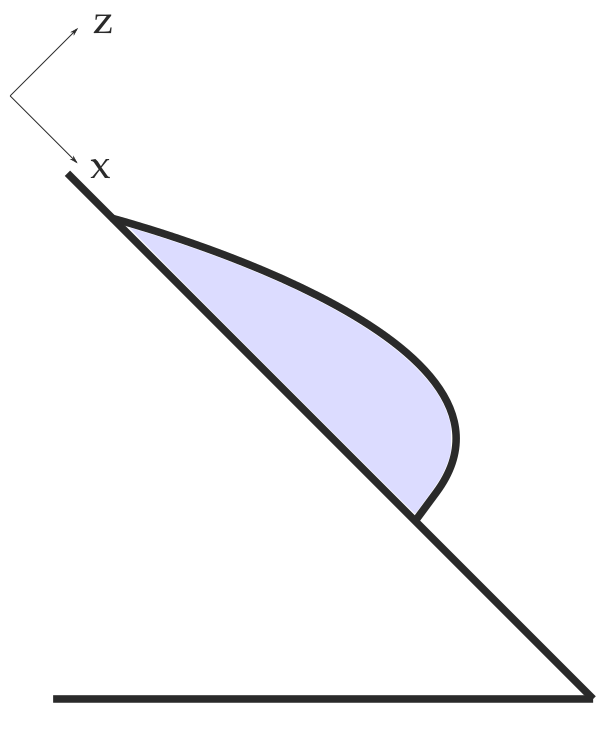
\includegraphics[scale = 0.2]{Figs/pendant_droplet_incline.png}
    \caption{Pendant droplet on an incline}
    \label{fig:pendant_droplet}
\end{figure}
The dimensional governing equations can be written as:
\begin{align}\label{eq:pendant_gov_eqns_dim}
 \begin{split}
  \frac{\partial p}{\partial x} &= \mu \frac{\partial^{2} u}{\partial z^{2}} + \rho g \sin{\alpha}\\
  \frac{\partial p}{\partial z} &= \mu \frac{\partial^{2} w}{\partial z^{2}} - \rho g \cos{\alpha}\\
  \frac{\partial u}{\partial x} + \frac{\partial w}{\partial z} &= 0.
 \end{split}
\end{align}
and the dimensional boundary conditions (BCs) are:
\begin{align}\label{eq:pendant_bcs_dim}
 \begin{split}
  & u = w = 0 \quad  \textrm{at} \quad z = 0,\\
  %
  &\textrm{kinematic BC:} \quad \frac{D(z-h)}{Dt} = 0 \Rightarrow \quad w =\cancelto{0 \because \textrm{steady}}{\partial_{t} h} + u \partial_{x}h \quad  \textrm{at} \quad z = h(x),\\
  %
  & \textrm{Dynamic BC (tangential):} \quad t_{i}\sigma_{ij}n_{j} - \cancelto{0}{t_{i}{\sigma_{a}}_{ij} n_{j} } = \cancelto{0}{\frac{\partial \gamma}{\partial s}} \Rightarrow (\partial_{z}u + \partial_{x}w)(1-(\partial_{x})h^{2}) - 4 \partial_{x}h\partial_{x}u  = 0 \quad \\
  %
  & \textrm{at} \quad z = h(x),\\
  %
  & \textrm{Dynamic BC (normal):}n_{i}\sigma_{ij}n_{j} - \cancelto{p_{0}}{n_{i}{\sigma_{a}}_{ij} n_{j} } = \gamma K \quad \textrm{at} \quad z = h(x),\\
%   p - p_{0} \approx \gamma \partial_{xx} h \quad & \textrm{at} \quad z = h(x),
 \end{split}
\end{align}

Let us non-dimensionalize the governing equations and BCs. 

The scalings used are as follows:
\begin{equation}\label{eq:pendant_scalings}
 x \sim L, z \sim h, u \sim U, w \sim W, p \sim P
\end{equation}
From the continuity equation $O(\partial_{x}u) \sim O(\partial_{z}w)$ for balancing each other. 

This immediately yields the scaling for $W$ in terms of $U$, i.e. 
\begin{align}\label{eq:pendant_w_scale}
 \begin{split}
  \frac{U}{L} &\sim \frac{W}{h_{0}},\\
  \Rightarrow W &\sim \frac{Uh_{0}}{L} = \epsilon U.
 \end{split}
\end{align}
where $\epsilon = h_{0}/L \ll 1 $ is the thin-film approximation. We now turn to the $x$-momentum equation to obtain the scale for pressure in terms of $U$. Balancing the pressure gradient and the viscous terms, we obtain
\begin{align}\label{eq:pendant_p_scale}
 \begin{split}
  \frac{P}{L} &\sim \frac{\mu U}{h^{2}},\\
  P & \sim \frac{\mu U L}{h^{2}} = \frac{\mu U}{\epsilon^{2}L}.
 \end{split}
\end{align}

We now turn to the normal stress boundary condition at $z = h(x)$. As shown in class, the normal stress boundary condition at the leading order reduces to the so called Young-Laplace equation $p - p_{0} = -\epsilon^{3} \bar{c}^{-1} \partial^{2}_{x}h$, where all the variables are dimensionless and $\bar{c} = \frac{\mu U}{\gamma}$ is the capillary number. In order to retain the effects of surface tension at the leading order, we demand $\epsilon^{3} \bar{c}^{-1} = O(1)$. Specifically, re-scaling $\epsilon^{-3} \bar{c} = C$, where $C = O(1)$ is the new capillary number. This yields the scaling for $u$,
\begin{align}\label{eq:pendant_u_scale}
 \begin{split}
  C &= \bar{c}/\epsilon^{3},\\
  &= \mu U/\gamma \epsilon^{3},\\
  U &\sim \gamma \epsilon^{3}/\mu.
 \end{split}
\end{align}

Using these scales, the dimensionless governing equations and boundary conditions become: 
\begin{align}\label{eq:pendant_gov_eqns_dimless_0}
 \begin{split}
    \frac{\partial p}{\partial x} &= \frac{\partial^{2} u}{\partial z^{2}} + (\rho g  L^{2} \sin{\alpha}/ \gamma\epsilon)\\
  \frac{\partial p}{\partial z} &= \epsilon^{2} \frac{\partial^{2} w}{\partial z^{2}} - (\rho g L^{2} \cos{\alpha}/ \gamma) \\
  \frac{\partial u}{\partial x} + \frac{\partial w}{\partial z} &= 0.
 \end{split}
\end{align}
Defining $G = \rho g L^{2}/\gamma$ to be the ``gravity'' number, we obtain

\begin{align}\label{eq:pendant_gov_eqns_dimless}
 \begin{split}
 \frac{\partial p}{\partial x} &= \frac{\partial^{2} u}{\partial z^{2}} + \frac{G \sin{\alpha}}{\epsilon}\\
  \frac{\partial p}{\partial z} &= \epsilon^{2} \frac{\partial^{2} w}{\partial z^{2}} - G \cos{\alpha} \\
  \frac{\partial u}{\partial x} + \frac{\partial w}{\partial z} &= 0.
 \end{split}
\end{align}
And the BCs become:

\begin{align}\label{eq:pendant_bcs_dimless}
 \begin{split}
  & u = w = 0 \quad \textrm{at} \quad z = 0,\\
  %
  & w = u h_{x} \quad \textrm{at} \quad z = h(x),\\
  %
  & u_{z} = 0 \quad \textrm{at} \quad z = h(x),\\
  % 
  & p - p_{0} = -C ^{-1}h_{xx} \quad \textrm{at} \quad z = h(x),\\
  & h = 0, \quad \textrm{at} \quad x = 0, 1.
 \end{split}
\end{align}

At the leading order, the $z$-momentum equation becomes $p_{z} = -G\cos{\alpha}$, which is just hydrostatic balance. Integrating wrt $z$, we get:
\begin{equation}
 p = -[G\cos{\alpha} ]z + \tilde{p}(x),
\end{equation}
where $\tilde{p}(x)$ is a constant of integration. Applying the normal-stress BC (the Young-Laplace condition), we obtain, $p|_{h} = p_{0} - C^{-1}h_{xx}$. 
\begin{align}\label{eq:pendant_get_p}
 \begin{split}
  p_{0} - h_{xx} &= -[G\cos{\alpha}] h + \tilde{p}(x),\\
  \Rightarrow \tilde{p}(x) &= p_{0} + [G\cos{\alpha}] h - C^{-1}h_{xx}\\
  \Rightarrow p &= p_{0} + [G\cos{\alpha}](h - z) - C^{-1}h_{xx}.\\
 \end{split}
\end{align}

Therefore, $\boxed{p = p_{0} + [G\cos{\alpha}](h - z) - C^{-1}h_{xx}}$.

Substituting in the $x$-momentum equation and integrating wrt z twice, obtain $u$:

\begin{align}\label{eq:pendant_get_u}
 \begin{split}
 & \int_{z=0}^{z} \left[(G\cos{\alpha})h_{x} - C^{-1}h_{xxx} = u_{zz} +  \frac{G\sin{\alpha}}{\epsilon}\right] dz,\\
% 
& u_{z} = \left[(G\cos{\alpha}) h_{x} - C^{-1}h_{xxx} - \frac{G\sin{\alpha}}{\epsilon}\right] z + \tilde{u_{z}}(x),\\ 
& \because u_{z} = 0 \quad \textrm{at} \quad z = h(x), \\
 \tilde{u_{z}}(x) & = -\left[(G\cos{\alpha}) h_{x} - C^{-1}h_{xxx} - \frac{G\sin{\alpha}}{\epsilon}\right]h ,\\
 & \boxed{u_{z} = \left[(G\cos{\alpha}) h_{x} - C^{-1}h_{xxx} - \frac{G\sin{\alpha}}{\epsilon}\right](z-h)},\\
 & \Rightarrow u = \left[(G\cos{\alpha}) h_{x} - C^{-1}h_{xxx} - \frac{G\sin{\alpha}}{\epsilon}\right]\left(\frac{z^{2}}{2} - hz \right) + \tilde{u}(x),\\
 & \because u = 0 \quad \textrm{at} \quad z = 0, \\
 & \tilde{u} = 0,\\
 & \Rightarrow \boxed{u = \left[(G\cos{\alpha}) h_{x} - C^{-1}h_{xxx} - \frac{G\sin{\alpha}}{\epsilon}\right]\left(\frac{z^{2}}{2} - hz \right)}.
 \end{split}
\end{align}
%--------------------------
% Substituting in the continuity equation and integrating wrt $z$, we get $w$:
% \begin{align}\label{eq:pendant_get_w}
%  \begin{split}
% & w_{z} = - \left[\frac{B\cos{\alpha}}{C} h_{xx} - h_{xxxx} \right]\left(\frac{z^{2}}{2} - hz \right) -  \left[\frac{B\cos{\alpha}}{C} h_{x} - h_{xxx} - \frac{B\sin{\alpha}}{C\epsilon}\right]\left(- h_{x}z \right)\\
% %
% & w_{z} = \left[\frac{B\cos{\alpha}}{C} ((h_{x})^{2} + h h_{xx}) - h_{x}h_{xxx} - \frac{B\sin{\alpha}}{C\epsilon} h_{x}  - h h_{xxxx}\right] z - \left[\frac{B\cos{\alpha}}{C} h_{xx} - h_{xxxx} \right]\frac{z^{2}}{2}, \\
% %
% & \Rightarrow w = \left[\frac{B\cos{\alpha}}{C} ((h_{x})^{2} + h h_{xx}) - h_{x}h_{xxx} - \frac{B\sin{\alpha}}{C\epsilon} h_{x}  - h h_{xxxx}\right] \frac{z^{2}}{2} - \left[\frac{B\cos{\alpha}}{C} h_{xx} - h_{xxxx} \right]\frac{z^{3}}{6} + \tilde{w}(x),\\
% %
% & \because w = 0 \quad \textrm{at} \quad z = 0, \quad \tilde{w}(x) = 0,\\
% %
% & \boxed{w = \left[\frac{B\cos{\alpha}}{C} ((h_{x})^{2} + h h_{xx}) - h_{x}h_{xxx} - \frac{B\sin{\alpha}}{C\epsilon} h_{x}  - h h_{xxxx}\right] \frac{z^{2}}{2} - \left[\frac{B\cos{\alpha}}{C} h_{xx} - h_{xxxx} \right]\frac{z^{3}}{6}}.
%  \end{split}
% \end{align}
% 
% Finally, applying the kinematic BC at $z=h$, we get the equation solely in terms of $h$.
% \begin{align}\label{eq:pendant_get_h}
% \begin{split}
%  &\left[\frac{B\cos{\alpha}}{C} ((h_{x})^{2} + h h_{xx}) - h_{x}h_{xxx} - \frac{B\sin{\alpha}}{C\epsilon} h_{x}  - h h_{xxxx}\right] \frac{h^{2}}{2} - \left[\frac{B\cos{\alpha}}{C} h_{xx} - h_{xxxx} \right]\frac{h^{3}}{6} \\
%  & = -\left[\frac{B\cos{\alpha}}{C} h_{x} - h_{xxx} - \frac{B\sin{\alpha}}{C\epsilon}\right]\frac{h^{2}h_{x}}{2},\\
%  %
%  & \left[\frac{B\cos{\alpha}}{C} (h_{x})^{2} -  h_{x}h_{xxx} - \frac{B\sin{\alpha}}{C\epsilon} h_{x}\right]h^{2} +   \left[\frac{B\cos{\alpha}}{C} hh_{xx} - h_{x}h_{xxx} - \frac{B\sin{\alpha}}{C\epsilon} h_{x}\right]\frac{h^{2}}{2}\\
%  & - \left[\frac{B\cos{\alpha}}{C} h_{xx} - h_{xxxx} \right]\frac{h^{3}}{6} = 0.
% \end{split} 
% \end{align}
%--------------------------
Now, integrating continuity equation across the domain wrt $z$, we obtain:
\begin{align}\label{eq:pendant_integrate_conti}
\begin{split}
 \int_{z=0}^{h(x)} [\partial_{x} u + \partial_{z} w_{z} &= 0 ] dz,\\
 w\big|_{0}^{h} + \int_{z=0}^{h(x)} \partial_{x} u dz &= 0,\\
 \cancelto{0 \because \textrm{steady}}{\partial_{t}h} + u|_{h} \partial_{x}h - 0 +  \int_{z=0}^{h(x)} (\partial_{x} u )dz &= 0 \quad \hdots \textrm{using BCs for } w, \\
 \cancel{u|_{h} \partial_{x}h} + \partial_{x} \int_{z=0}^{h(x)} u dz - \cancel{u|_{h} \partial_{x}h} &= 0 \quad \hdots \textrm{Leibniz rule},\\
 \int_{z=0}^{h(x)} u dz = c\\
\end{split}
\end{align}

However, $Q = \int_{z=0}^{h(x)} u dz$ corresponds to the volume flux and there is no volume flux here. So $c = 0$. We then get the equation for $h$.

\begin{align}\label{eq:get_h}
 \begin{split}
  \int_{0}^{h}\left[(G\cos{\alpha}) h_{x} - C^{-1}h_{xxx} - \frac{G\sin{\alpha}}{\epsilon}\right]\left(\frac{z^{2}}{2} - hz \right) dz &= 0\\
  %
  \left[(G\cos{\alpha}) h_{x} - C^{-1}h_{xxx} - \frac{G\sin{\alpha}}{\epsilon}\right]\left(\frac{z^{3}}{6} - h\frac{z^{2}}{2} \right)\bigg|_{0}^{h} &= 0\\
  %
  (G\cos{\alpha}) h_{x} - C^{-1}h_{xxx} - \frac{G\sin{\alpha}}{\epsilon} &= 0.
 \end{split}
\end{align}

For gravity to do anything, it must have an $O(1)$ effect in the $x$-direction. Redefining $\tilde{G} = G/\epsilon$ and demanding $\tilde{G} \sim O(1)$, we get
\begin{equation}\label{eq:rescale_G}
 (\epsilon \tilde{G}\cos{\alpha}) h_{x} - C^{-1}h_{xxx} - \tilde{G}\sin{\alpha} = 0.
\end{equation}

Neglecting the $O(\epsilon)$ term at the leading order, we obtain
\begin{equation}\label{eq:pendant_h}
 C^{-1}h_{xxx} + \tilde{G}\sin{\alpha} = 0
\end{equation}

Finally defining the Bond number to be $B = \tilde{G} C = \rho g L^{2} C/\epsilon \gamma$, and integrating thrice in $x$, we get:
\begin{align}\label{eq:pendant_integrate_h}
 h_{xxx} &= (-B \sin{\alpha})\\
 h_{xx}  &= (-B \sin{\alpha}) x + c_{1}\\
 h_{x}   &=(-B \sin{\alpha}) \frac{x^{2}}{2} + c_{1} x + c_{2}\\
 h &= (-B \sin{\alpha}) \frac{x^{3}}{6} + c_{1} \frac{x^{2}}{2} + c_{2} x + c_{3}
\end{align}

Since $h = 0$ at $x=0, 1$, $c_{3} = 0$ and $c_{1}/2 + c_{2} = B\sin{\alpha}/6$. Hence, $h = (-B \sin{\alpha}) \frac{x^{3}}{6} + c_{1} \frac{x^{2}}{2} + c_{2} x$. 

Also, the volume $V_{0}$ is preserved. In dimensionless terms $V_{0} = \int_{0}^{1} hdx$.
Therefore, we get, 
\begin{equation}\label{eq:pendant_conserve_V}
 V_{0} = -B\sin{\alpha}/24 + c_{1}/6 + c_{2}/2
\end{equation}

Solving 
$c_{1}/2 + c_{2} = B\sin{\alpha}/6$ and Eqn.(\ref{eq:pendant_conserve_V}) simultaneously, we obtain: $c_{1} =  \frac{-24V_{0} + B\sin{\alpha}}{2}$ and $c_{2} = \frac{72 V_{0} - B\sin{\alpha}}{12}$.  

%----------------------------------------------
\section{Q $3$: Linear stability of a liquid film with non-uniform surface tension and destabilizing gravity. }
%----------------------------------------------
%-----------
\subsection*{Governing Equations and BCs:}
%-----------
The governing equations, as before, can be written as 
\begin{align}\label{eq:marangoni_gov_eqns_dimless}
 \begin{split}
 \frac{\partial p}{\partial x} &= \frac{\partial^{2} u}{\partial z^{2}}  \\
  \frac{\partial p}{\partial z} &= \epsilon^{2} \frac{\partial^{2} w}{\partial z^{2}} - G  \\
  \frac{\partial u}{\partial x} + \frac{\partial w}{\partial z} &= 0.
 \end{split}
\end{align}
These can be easily retrieved from Eqns.(\ref{eq:pendant_gov_eqns_dimless}) by setting $\alpha = 0$. Here, $G = \rho g L^{2}/\gamma_{0}$ as defined in the previous problem. 

The tangential stress boundary condition can be written as follows:
\begin{align}\label{eq:tangential_stress_bc}
 \begin{split}
  t_{i}\sigma_{ij}n_{j} - t_{i}\cancelto{0}{{\sigma_{a}}_{ij}}n_{j} &= \partial_{s}\gamma \quad s\textrm{is the arclength along the surface},\\
  \hat{t} = \frac{\hat{e}_{x} + \partial_{x}h\hat{e}^{z}}{\sqrt{1+ (\partial_{x}h)^{2}}}, & \quad \hat{n} = \frac{-\partial_{x}h\hat{e}_{x} + \hat{e}^{z}}{\sqrt{1+ (\partial_{x}h)^{2}}}\\
  \therefore t_{1}\sigma_{11}n_{1} + t_{1}\sigma_{12}n_{2} + t_{1}\sigma_{12}n_{2} + t_{2}\sigma_{22}n_{2} &= \partial_{s}\gamma\\  
  \mu(\partial_{z}u + \partial_{x}w)(1 - (\partial_{x}h)^{2}) - 4\mu \partial_{x}h(\partial_{x}u - \partial_{z}w) &= \partial_{s}\gamma.
 \end{split}
\end{align}
But $ds \approx \sqrt{dx^{2} + dy^{2}} = dx (\sqrt{1 + (\partial_{x}h)^{2}})$ at $y=h$.
This gives $\partial_{s} = \frac{\partial_{x}}{\sqrt{1 + (\partial_{x}h)^{2}} }$.
In dimensionless terms, using the scaling for $u$ from Eqn. (\ref{eq:pendant_u_scale}), $U \sim \gamma_{0} \epsilon^{3}/\mu$ we get:
%
\begin{align}\label{eq:marangoni_tangential_stress_bc}
\begin{split}
& \frac{1}{1 + \epsilon^{2}(\partial_{x}h)^{2}}\left[\mu (\partial_{z}u + \partial_{x}w)(1 - \epsilon^{2}(\partial_{x}h)^{2}) U/(L\epsilon) - 4\mu \partial_{x}h(\partial_{x}u - \partial_{z} w) \epsilon U/L \right]\\
%
&= (\gamma_{0}/L) \frac{\partial_{x}\gamma}{\sqrt{1 + (\partial_{x}h)^{2}}},\\
%
& \frac{1}{\sqrt{1 + \epsilon^{2}(\partial_{x}h)^{2}}}\left[\mu (\partial_{z}u + \partial_{x}w)(1 - \epsilon^{2}(\partial_{x}h)^{2}) (\gamma_{0} \epsilon^{3}/\mu)/(\epsilon) - 4\mu \partial_{x}h(\partial_{x}u - \partial_{z} w) \epsilon (\gamma_{0} \epsilon^{3}/\mu) \right]\\
%
&= \gamma_{0} \partial_{x}\gamma,\\
%
& \boxed{\epsilon^{2} \partial_{z} u = \partial_{x}\gamma } \quad \textrm{at the leading order}.
\end{split}
\end{align}
Writing $\gamma = 1 + \epsilon^{2}\gamma$ and equating terms of the same order in $\epsilon$, the tangential BC at the leading order reduces to $\boxed{\partial_{z}u = \partial_{x}\gamma_{1}}$. 
Also, the dynamic boundary condition (in the normal direction), in dimensional terms is the Young-Lapace equation $p-p_{0} = -\gamma \partial^{2}_{x}$. In dimensionless terms, we remember that $\gamma$ is no longer a constant. The dimensionless version will read $p - p_{0} = C^{-1}\gamma \partial_{x}^{2}h$, where all the quantities are now dimensionless. 

Hence the BCs become:
\begin{align}\label{eq:marangoni_bcs_dimless}
 \begin{split}
  & u = w = 0 \quad \textrm{at} \quad z = 0,\\
  %
  & w = \partial_{t}h + u \partial_{x} x \quad \textrm{at} \quad z = h(x),\\
  %
  & u_{z} = (\partial_{x}\gamma_{1}) \quad \textrm{at} \quad z = h(x),\\
  % 
  & p - p_{0} = -C^{-1} (1 + \epsilon^{2}\gamma_{1})\partial_{x}^{2}h \quad \textrm{at} \quad z = h(x),\\
  & h = 0, \quad \textrm{at} \quad x = 0, 1.
 \end{split}
\end{align}
As before, integrating the $z$-momentum equation at the leading order is just the hydrostatic balance. Integrating the $z$-momentum equation in $z$, we obtain the pressure distribution. This is similar to the previous question and we directly write $p$, by setting $\alpha = 0$ in Eqn.(\ref{eq:pendant_get_p}). 
\begin{equation}\label{eq:marangoni_p}
 p = p_{0} + G(h-z) - C^{-1}(1 + \epsilon^{2}\gamma_{1})h_{xx}.
\end{equation}
Let us define $\pi = p - p_{0}$ to be the gauge pressure. Therefore, $\pi = G(h-z) - C^{-1}h_{xx}$.\\
Substituting in the $x$-momentum equation and integrating twice wrt $z$, we get:
\begin{align}\label{eq:marangoni_u}
 \begin{split}
  & \partial^{2}_{z}u = \partial_{x}\pi \quad  \hdots \because \partial_{x}p = \partial_{x}\pi \\
  %
  \Rightarrow \quad & \partial_{z}u = (\partial_{x}\pi)z + c_{1}(x, t)\\
  %
  & \partial_{z} u = (\partial_{x}\gamma_{1}) \quad \textrm{at} \quad z = h(x),\\
  %
  \Rightarrow \quad & u_{z} = (\partial_{x}\pi)(z-h) + (\partial_{x}\gamma_{1})\\
  %
  \Rightarrow \quad & u =  (\partial_{x}\pi)\left(\frac{z^{2}}{2}-hz\right) + (\partial_{x}\gamma_{1})z + c_{2}(x, t)\\
  & u = 0 \quad \textrm{at} \quad z = 0 \Rightarrow c_{2}(x, t) = 0.\\
  \Rightarrow \quad & \boxed{ u =  (\partial_{x}\pi)\left(\frac{z^{2}}{2}-hz\right) + (\partial_{x}\gamma_{1})z }.
 \end{split}
\end{align}
Substituting into conservation of mass Eqn.(\ref{eq:pendant_integrate_conti}),
\begin{align}
 \begin{split}
 & \partial_{t} h + \partial_{x}\int_{0}^{h(x)} \partial_{x}\pi \left( \frac{z^{2}}{2} - hz \right) +  (\partial_{x}\gamma_{1})z dz = 0 \\
 %
 & \partial_{t} h + \partial_{x}\left[ \partial_{x}\pi \left(\frac{z^{3}}{6}  - \frac{hz^{2}}{2}\right) + (\partial_{x}\gamma_{1}) \frac{z^{2}}{2} \right]_{0}^{h}= 0\\
 %
 & \partial_{t} h + \partial_{x}\left[(\partial_{x}\gamma_{1})\frac{h^{2}}{2} - (\partial_{x}\pi) \frac{h^{3}}{3}  \right] = 0\\
 %
 & \partial_{t} h + \partial_{x}\left[(\partial_{x}\gamma_{1})\frac{h^{2}}{2} - \left( G\partial_{x}h - C^{-1} (1 + \epsilon^{2}\gamma_{1}) \partial_{x}^{3} h -\epsilon^{2} C^{-1} (\partial_{x}\gamma_{1})( \partial^{2}_{x}h)\right) \frac{h^{3}}{3}  \right] = 0.\\
 \end{split}
\end{align}

Rescaling time to $T = t/C$, old time scale $U_{0}/L$ changes to $T = t'/(\mu L/\epsilon^{3}\gamma_{0})$, where $t'$ is the dimensional time. Also, defining $CG = C\rho g L^{2}/\gamma_{0}$ to be the ``Bond number'', we obtain:
\begin{align}\label{eq:marangoni_h}
\begin{split}
 & \partial_{T}h + \partial_{x}\left[C(\partial_{x}\gamma_{1})\frac{h^{2}}{2} - \left( B\partial_{x}h -  (1 + \epsilon^{2}\gamma_{1}) \partial_{x}^{3} h -\epsilon^{2} (\partial_{x}\gamma_{1})( \partial^{2}_{x}h) \right) \frac{h^{3}}{3}  \right] = 0.\\
 %
 & \textrm{at the leading oredr } O(1) \\
 %
 &\boxed{\partial_{T}h + \partial_{x}\left[C(\partial_{x}\gamma_{1})\frac{h^{2}}{2} - \left( B\partial_{x}h -  \partial_{x}^{3} h \right) \frac{h^{3}}{3}  \right] = 0 }.
\end{split}
\end{align}

%-----------
\subsection*{Linear stability of a uniformly thick film lining the underside of a rigid flat horizontal substrate}
%-----------
\begin{figure}[H]
    \centering
    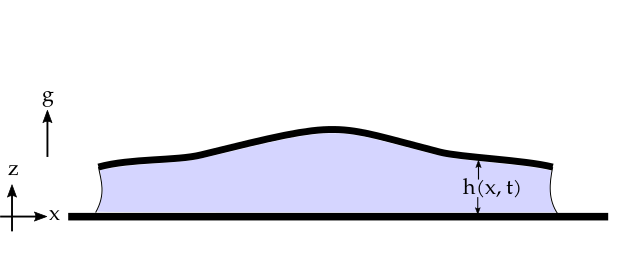
\includegraphics[scale = 0.5]{Figs/marangoni.png}
    \caption{A film lining the underside of a rigid flat horizontal substrate.}
    \label{fig:marangoni_underside}
\end{figure}

We say that a film lining underside of a rigid horizontal substrate is equivalent to the case of regular film on a horizontal substrate, with gravity pointing upwards. So we let $B\rightarrow -B$, and $\gamma_{1} = \Lambda/h$ ($\Rightarrow \partial_{x}\gamma_{1} = \frac{-\Lambda}{h^{2}} \partial_{x}h$), we get:

\begin{equation}\label{eq:marangoni_gov_eqn}
 \partial_{T}h + \partial_{x}\left[-\frac{C\Lambda}{2} \partial_{x}h + \left( B\partial_{x}h + \partial_{x}^{3} h \right) \frac{h^{3}}{3}  \right] = 0
\end{equation}
The base state is $h_{b} = 1$. Introduce a perturbation of the form $h = 1 + \eta$. Substituting in Eqn.(\ref{eq:marangoni_gov_eqn}), obtain:

\begin{align}\label{eq:marangoni_perturbation_eqn}
 \begin{split}
  &\partial_{T}\eta + \partial_{x}\left[-\frac{C\Lambda}{2} \partial_{x}\eta + \left( B\partial_{x}\eta + \partial_{x}^{3} \eta \right) \frac{1}{3}  \right] = 0,\\
  %
  &\partial_{T}\eta + \frac{1}{3}\partial^{4}_{x}\eta + \frac{B}{3} \partial^{2}_{x}\eta - \frac{C\Lambda}{2}\partial^{2}_{x}\eta = 0.
 \end{split}
\end{align}
Now, we start by ``modal analysis'', i.e., seek solutions of the form $\eta = A e^{\sigma t} e^{ikx} + \textrm{c.c.}$ where $k$ is the (known) real wavenumber of the perturbation, $\sigma$ is the possibly complex growth rate and c.c. denotes the complex conjugate. Substituting into Eqn.(\ref{eq:marangoni_perturbation_eqn}):
\begin{equation}
 \sigma + \frac{k^{4}}{3} - \left(\frac{B}{3} -\frac{C\Lambda}{2}\right) k^{2} = 0
\end{equation}

Hence, we get the dispersion relation $\sigma \equiv \sigma(k)$. 
\begin{equation}\label{eq:marangoni_dispersion_reln}
 \sigma =  \left(\frac{B}{3} -\frac{C\Lambda}{2}\right) k^{2} - \frac{k^{4}}{3}
\end{equation}

Unstable when $Re(\sigma) > 0$. 

\begin{figure}[H]
    \centering
    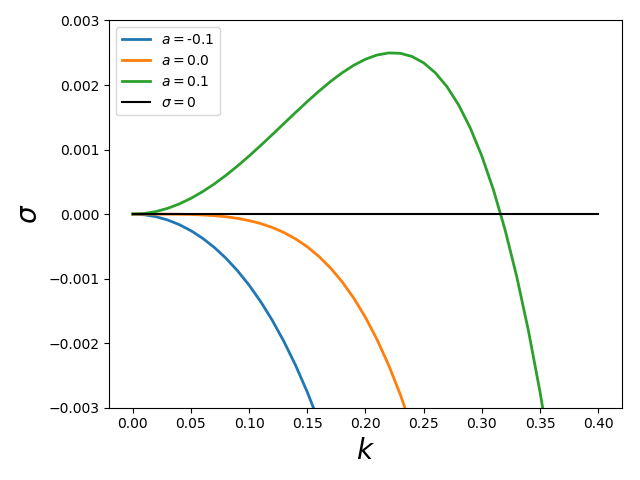
\includegraphics[scale = 0.5]{Figs/marangoni_dispersion_reln.png}
    \caption{Dispersion relation ($\sigma \equiv \sigma(k)$) for the inear stability of a uniformly thick film lining the underside of a rigid flat horizontal substrate with $a = 2B - 3C\Lambda$ }
    \label{fig:marangoni_dispersion_reln}
\end{figure}
From Fig.(\ref{fig:marangoni_dispersion_reln}), it is clear that when $a>0$, a band of modes become unstable. Hence, the condition for instability is $2B - 3C\Lambda \geq 0$ or $\boxed{B > 3C\Lambda/2}$.

%----------------------------------------------
\section{Q $4$: Marangoni convection in the inertia-less limit: }
%----------------------------------------------
The aim of the analysis is to investigate the possibility that, even in the absence of buoyancy, convection may be possible provided that the temperature-dependence of the surface tension coefficient $\gamma$ is accounted for.

The dimensional governing equations are the incompressible Stokes equations w/o gravity:
\begin{align}\label{eq:marangoni_convect_gov_eqns_dim_1}
 \begin{split}
  &\partial_{x}p = \mu (\partial^{2}_{x}u +\partial^{2}_{z}u),\\
  %
  &\partial_{z}p = \mu (\partial^{2}_{x}w +\partial^{2}_{z}w),\\
  %
  & 0 = \partial_{x}u + \partial_{z} w, \\
  %
  & \partial_{t}T + u \partial_{x}T + w \partial_{z} T = \kappa (\partial^{2}_{x}T +\partial^{2}_{z}T),\\
 \end{split}
\end{align}

The BCs are:
\begin{align}
\label{eq:marangoni_convect_bcs_dim_1}
 \begin{split}
  & u = w = 0 \quad \textrm{at } z = 0,\\
  %
  & \mu \partial_{z}u = \partial_{x}\gamma \quad \textrm{at } z = H,\\
  %
  \textrm{where}\quad & \gamma = \gamma_{0}-\Lambda(T-T_{0}),\\
  %
  & w = 0 \quad \textrm{at } z = H, \\
  %
  & T=T_{0} \quad \textrm{at } z = 0, \\
  %
  & \partial_{z}T = -Q_{0} \quad \textrm{at } z = H.
 \end{split}
\end{align}

The surface height $H$ remains constant throughout this analysis. 

First, we cast the governing equations in terms of the streamfunction $\psi$, such that 
\begin{equation}\label{eq:streamfunction_def}
 u = \partial_{z}\psi,\quad w = -\partial_{x}w.
\end{equation}
The incompressibility condition is then automatically satisfied. Eliminating pressure  by taking the curl of the momentum equations:
\begin{align}
 \begin{split}
  & \mu(\partial^{2}_{x} \partial_{z} u + \partial^{3}_{z} u - \partial^{3}_{x}  w - \partial^{2}_{z}\partial_{x} w)  = 0,\\
  %
  \Rightarrow \quad & (\partial^{4}_{x} + 2\partial^{2}_{x}\partial^{2}_{z} + \partial^{4}_{z})\psi = 0,\\
  %
  & \boxed{\nabla^{4}\psi = 0}.
 \end{split}
\end{align}


The dimensional equations and BCs, in terms of the streamfunction $\psi$ can be written as:
\begin{align}\label{eq:marangoni_convect_gov_eqns_dim}
 \begin{split}
  &\nabla^{4}\psi = 0, \\
  & \partial_{t}T + [u \cdot \nabla]T  = \kappa \nabla^{2}T.
 \end{split}
\end{align}

The BCs become:
\begin{align}
 \label{eq:marangoni_convect_bcs_dim}
 \begin{split}
  & \partial_{z}\psi = \partial_{x}\psi = 0 \quad \textrm{at } z = 0,\\
  %
  & \mu \partial_{zz} \psi = \partial_{x}\gamma \quad \textrm{at } z = H,\\
  %
  \textrm{where}\quad & \gamma = \gamma_{0}-\Lambda(T-T_{0}),\\
  %
  & \partial_{x}\psi = 0 \quad \textrm{at } z = H, \\
  %
  & T=T_{0} \quad \textrm{at } z = 0, \\
  %
  & \partial_{z}T = -Q_{0} \quad \textrm{at } z = H.
 \end{split}
\end{align}

Scaling $x\sim H, y\sim H, u \sim \kappa/H, T\sim Q_{0}H$, we obtain scalings for time and streamfunction. The scaling for time is obtained from the energy equation, where $\partial_{t}T$ must balance $\kappa \nabla^{2}T$, yielding $t \sim H^{2}/\kappa$. From the definition of the streamfunction, we get $\psi \sim  \kappa$. Using these scales, we obtain the dimensionless equations:
\begin{align}
\label{eq:marangoni_convect_gov_eqns_dimless}
 \begin{split}
  &\nabla^{4}\psi = 0, \\
  & \partial_{t}T + [u \cdot \nabla]T  = \nabla^{2}T.
 \end{split}
\end{align}

The BCs become:
\begin{align}\label{eq:marangoni_convect_bcs_dimless}
 \begin{split}
  & \partial_{z}\psi = \partial_{x}\psi = 0 \quad \textrm{at } z = 0,\\
  %
  & \partial_{zz} \psi = -\tilde{\Lambda}\partial_{x}T 
  \quad \textrm{at } z = 1, \quad \textrm{where } \tilde{\Lambda} = \frac{\Lambda Q_{0}H^{2}}{\kappa \mu},\\
  %
  & \partial_{x}\psi = 0 \quad \textrm{at } z = 1, \\
  %
  & T=T_{0}/(Q_{0}H) \quad \textrm{at } z = 0, \\
  %
  & \partial_{z}T = -1 \quad \textrm{at } z = 1.
 \end{split}
\end{align}
All the quantities in the above BCs are now dimensionless. If $\psi = \textrm{ const}$, $\nabla^{4}\psi$ is definitely zero and $\boldsymbol{u}_{b}=\boldsymbol{0}$ is the base state velocity. Without loss of generality, we take $\boxed{\psi_{b} = 0}$. 
We assume a steady conduction base state for the temperature with no $x$-variation. $\partial_{zz}T_{b} = 0$, giving $T_{b} = Az + B$. With $T_{b}= T_{0}/(Q_{0}H) \quad \textrm{at } z = 0$, we get $B =T_{0}/(Q_{0}H)$ and $\partial_{z}T = -1 \quad \textrm{at } z = 1$ yields $A=-1$. Therefore, the steady state base temperature profile is $\boxed{T_{b} = T_{0}/(Q_{0}H) - z}$.  

Perturbing about the base state and substituting $\psi \equiv \psi_{b} + \psi$ and $T = T_{b} + \theta$ (noting that ${T_{b}}_{z} = -1$), into the governing equations and BCs,
\begin{align}\label{eq:perturbation_eqns}
 \begin{split}
  & \boxed{\nabla^{4}\psi = 0},\\
  %
  & \partial_{t}\theta + \psi_{z}\theta_{x} - \psi_{x}(-1 + \theta_{z}) = \nabla^{2}\theta. \\
  %
  & \textrm{Neglecting nonlinear terms}\\
  %
  &\boxed{\partial_{t}\theta + \psi_{x} = \nabla^{2}\theta}.
 \end{split}
\end{align}

The BCs become:
\begin{align}
\label{eq:perturbation_bcs}
 \begin{split}
  &\boxed{ \psi_{z} = \psi_{x} = \theta = 0} \quad \textrm{at } z = 0,  \\
  %
  & \boxed{ \psi_{x} = \theta_{z} = 0, \quad \psi_{zz} = -\tilde{\Lambda} \partial_{x}\theta} \quad \textrm{at } z = 1. 
 \end{split}
\end{align}

Substituting
\begin{equation}
 \begin{bmatrix}
    \theta \\
     \psi
 \end{bmatrix} = \begin{bmatrix}
    \hat{\theta} \\
     \hat{\psi}
 \end{bmatrix}e^{ikx}e^{\sigma t} + \textrm{c.c.}, 
\end{equation}

we obtain a linear eigenvalue problem in $z$.
\begin{align}
 \begin{split}
  & [k^{4} - 2k^{2}D^{2} + D^{4}] \hat{\psi} = 0\\
  & \sigma \hat{\theta} + ik \hat{\psi} = [-k^{2}+D^{2}]\hat{\theta}\\
  %
  & \textrm{combining the above, we obtain},\\
  %
  &\boxed{ \hat{\psi} = \frac{1}{ik} [-k^{2}+D^{2} - \sigma]\hat{\theta} }\quad \textrm{and}\\
  %
  & \boxed{ [D^{4} - 2k^{2}D^{2} + k^{4}][D^{2}-k^{2}]\hat{\theta} = \sigma [D^{4} - 2k^{2}D^{2} + k^{4}] \hat{\theta} },
 \end{split}
\end{align}

where $D \equiv d_{z}$. 

%----------------------------------------------
\section{Q $5$: A lubrication approximation for Darcy flow in semi-saturated porous media: }
%----------------------------------------------
Consider a $2d$ shallow-water flow over a porous medium of length $L$. The lubrication approximation here would be $\epsilon \equiv h/L \ll 1$.  We assume incompressibility and use Darcy's law as the momentum equations. The dimensional governing equations become:
\begin{align}
 \begin{split}
  & \boldsymbol{u} = -\frac{\kappa}{\mu}\nabla(p + \rho g z),\\
  %
  & \nabla.\boldsymbol{u} = 0.
 \end{split}
 \end{align}
%
In component form:
\begin{align}\label{eq:lub_darcy_flow_dim}
 \begin{split}
  & u = -\frac{\kappa}{\mu}\frac{\partial p}{\partial x},\\
  %
  & w = -\frac{\kappa}{\mu}\frac{\partial p}{\partial z} -\frac{\kappa \rho g}{\mu},\\
  %
  & \frac{\partial u}{\partial x} + \frac{\partial w}{\partial z} = 0.
 \end{split}
 \end{align}
%
 The boundary conditions are:
 \begin{align}\label{eq:lub_darcy_flow_bcs_dim}
  \begin{split}
   & w(x, z= 0, t) = 0,\\
   %
   & w(x, z= h(x,t), t) = \partial_{t}h + u \partial_{x}h,\\
   %
   & p(x, z=h(x,t), t) = p_{0},
  \end{split}
 \end{align}
%
where  $p_{0}$ is the constant atmospheric pressure impressed on the top of the groundwater layer (and
capillary effects are being neglected). Scaling $x \sim L, z \sim h, u \sim U, p \sim P$. The continuity equation implies $\frac{U}{L} \sim \frac{W}{h}$ or $W \sim Uh/L = \epsilon U$. The $x$-momentum equation implies $U \sim \kappa P/ \mu L \Rightarrow P \sim \mu U L/\kappa$. 
%
In the $z$-momentum equation, the relative size of $w$ and $ \frac{\kappa}{\mu}\frac{\partial p}{\partial z}$ term can be found to be:
\begin{align}
 \begin{split}
  & |w|\bigg/ \bigg|\frac{\kappa}{\mu}\frac{\partial p}{\partial z}\bigg| \sim \frac{\epsilon U}{UL/h},\\ 
  %
  &|w|\bigg/ \bigg|\frac{\kappa}{\mu}\frac{\partial p}{\partial z}\bigg| \sim \epsilon^{2}.
 \end{split}
\end{align}
%
Hence, we neglect $w$ at the leading order in the $z$-momentum equation. 
%
At the leading order, the dimensional $z$-momentum equation reads:
\begin{equation}
 \frac{\partial p}{\partial z} = -\rho g.
\end{equation}
Integrating, we obtain $p = -\rho g z + c(x)$. Using the boundary condition at the top surface $z=h$, obtain $ \boxed{ p - p_{0} = \rho g (h - z)}$.

Substituting in the $x$-momentum equation, obtain:
$\boxed{u = -\frac{\kappa \rho g}{\mu} \partial_{x}h}$.

Now, using the depth-averaged version of the continuity equation (see Eqns. (\ref{eq:integrate_conti}) and (\ref{eq:pendant_integrate_conti}))
\begin{align}
 \begin{split}
  & \partial_{t}h + \partial_{x}\left[ \int_{0}^{h} u dz\right] = 0,\\
  %
  & \partial_{t}h - \partial_{x}\left[ \frac{\kappa \rho g}{\mu} \partial_{x}h [z]_{0}^{h} \right] = 0,\\
  %
  & \partial_{t}h - \partial_{x}\left[ \frac{\kappa \rho g}{\mu} h \partial_{x}h \right] = 0,\\
  %
  & M \partial_{t}h = \partial_{x}\left[ h \partial_{x}h \right],\\
 \end{split}
\end{align}

where $M = \mu/(\kappa \rho g)$. This is nonlinear diffusion equation for $h(x, t)$. Notice that pressure and $h$ are linearly related in this problem. If there is a Gaussian pressure anomaly localized at $x=0$ at $t=0$, it will diffuse as time goes on. The time-scale for this would be governed by the above nonlinear diffusion equation. Namely, $ M/ t \sim h/L^{2}$ or $t \sim ML^{2}/h = ML/\epsilon$. This pressure diffusion is typical of porous media flows. 
%------------------------------------------------------
\bibliographystyle{apalike}
%\bibliographystyle{unsrt} % Use for unsorted references  
%\bibliographystyle{plainnat} % use this to have URLs listed in References
%\cleardoublepage
%\bibliography{References/references} % Path to your References.bib file

\bibliography{bib/references} % Path to your References.bib file
 \if@openright\cleardoublepage\else\clearpage\fi
 \cleardoublepage
 \pagestyle{empty}
%--------------------------------------------------------------------
\end{document}
